\documentclass[doc]{apa6}
\usepackage{amsmath}
\usepackage{hyperref}
\usepackage{csquotes}

\captionsetup{font=singlespacing,justification=justified}
\urlstyle{sf}


\title{Estimating evidential value from ANOVA summaries: A comment on Ly et al.~(2018)}
\author{Thomas J. Faulkenberry}
\date{}
\shorttitle{Estimating evidential value from ANOVA}
\affiliation{Tarleton State University}
\authornote{Correspondence concerning this article should be addressed to Thomas J. Faulkenberry, Department of Psychological Sciences, Box T-0820, Tarleton State University, Stephenville, TX 76401. E-mail: \href{mailto:faulkenberry@tarleton.edu}{\nolinkurl{faulkenberry@tarleton.edu}}}



\begin{document}
\maketitle

The last decade has witnessed a tremendous increase in the number of tools that enable social science researchers to perform Bayesian inference. Ly et al. (2018) recently described one such tool included as part of the open-source software package JASP -- the Summary Stats module (JASP Team, 2018). With this tool, researchers can input a minimal set of summary statistics (either from their own previously-run analysis or from the already published results of others) and obtain a Bayesian re-evaluation of the results. In particular, the Summary Stats module reports the Bayes factor (Kass \& Raftery, 1995), a continuous index of the extent to which observed data are more likely under one hypothesis (e.g., the null hypothesis \(\mathcal{H}_0\)) over another competing hypothesis (e.g., the alternative hypothesis \(\mathcal{H}_1\)). As a part of the Bayesian inferential framework, this Bayes factor (denoted \(B_{01}\)) describes the factor by which our prior relative belief between \(\mathcal{H}_0\) and \(\mathcal{H}_1\) should be updated after observing data. This characterization makes the Bayes factor a useful measure of the \emph{evidential value} of data (Etz \& Vandekerckhove, 2017).

As Ly et al. (2018) do an excellent job of describing, the JASP Summary Stats module is a powerful tool that gives the user access to some of the core elements of Bayesian inference without need for accompanying raw data. This provides users with flexibility; researchers may wish assess the evidential value of their own data to sensibly ground their interpretations, and reviewers/editors may wish to do the same for reported data to help with their own interpretations and decisions regarding publication. However, at present the Summary Stats module does not include an option for directly reanalyzing the results of an analysis of variance (ANOVA). ANOVA is often characterized as the \enquote{workhorse} of experimental psychology (Rouder, Engelhardt, McCabe, \& Morey, 2016). Thus, it would be quite helpful to the \enquote{academic consumer} to be able to to compute Bayes factors from minimal ANOVA summaries.

To this end, I wrote an interactive web application for calculating Bayes factors from minimal single factor ANOVA summaries (see Figure 1). The application, which can accessed by any web browser at \url{http://tomfaulkenberry.shinyapps.io/anovaBFcalc}, performs calculations that are based on the BIC method (Faulkenberry, 2018, 2019; Masson, 2011; Nathoo \& Masson, 2016; Wagenmakers, 2007). It requires minimal input; the user need only specify the \(F\) statistic and the degrees of freedom for the ANOVA. Additionally, the user may specify the design (between-subjects or repeated measures) and a prior probability for \(\mathcal{H}_0\) (default = 0.5). In return, the application provides the user with estimates of \(B_{01}\) and \(B_{10}\), a sentence interpreting what the Bayes factor means, a graphical display of the strength of evidence provided by the Bayes factor (i.e., a pizza plot\footnote{Please note that the pizza plot is designed to display the Bayes factor, not the posterior probabilities of $\mathcal{H}_0$ and $\mathcal{H}_1$. Consequently, it does not change when the user specifies a different prior probability for \(\mathcal{H}_0\). Instead, the pizza plot represents the weight of evidence {\it of the data} for one of the hypotheses over the other; in Figure 1, the slice for ``$\text{data}\mid \mathcal{H}_0$'' has 5.08 times more area than the slice for ``$\text{data}\mid \mathcal{H}_1$''. Regardless of a user's prior probability for \(\mathcal{H}_0\), the weight of evidence of the data is the same. That is, for both hypothetical users above, the prior odds between \(\mathcal{H}_0\) and \(\mathcal{H}_1\) have been increased by a factor of 5.08 after observing data.}, Wagenmakers et al., 2017), and estimates of the posterior probability of each hypothesis.

\begin{figure}
\centering
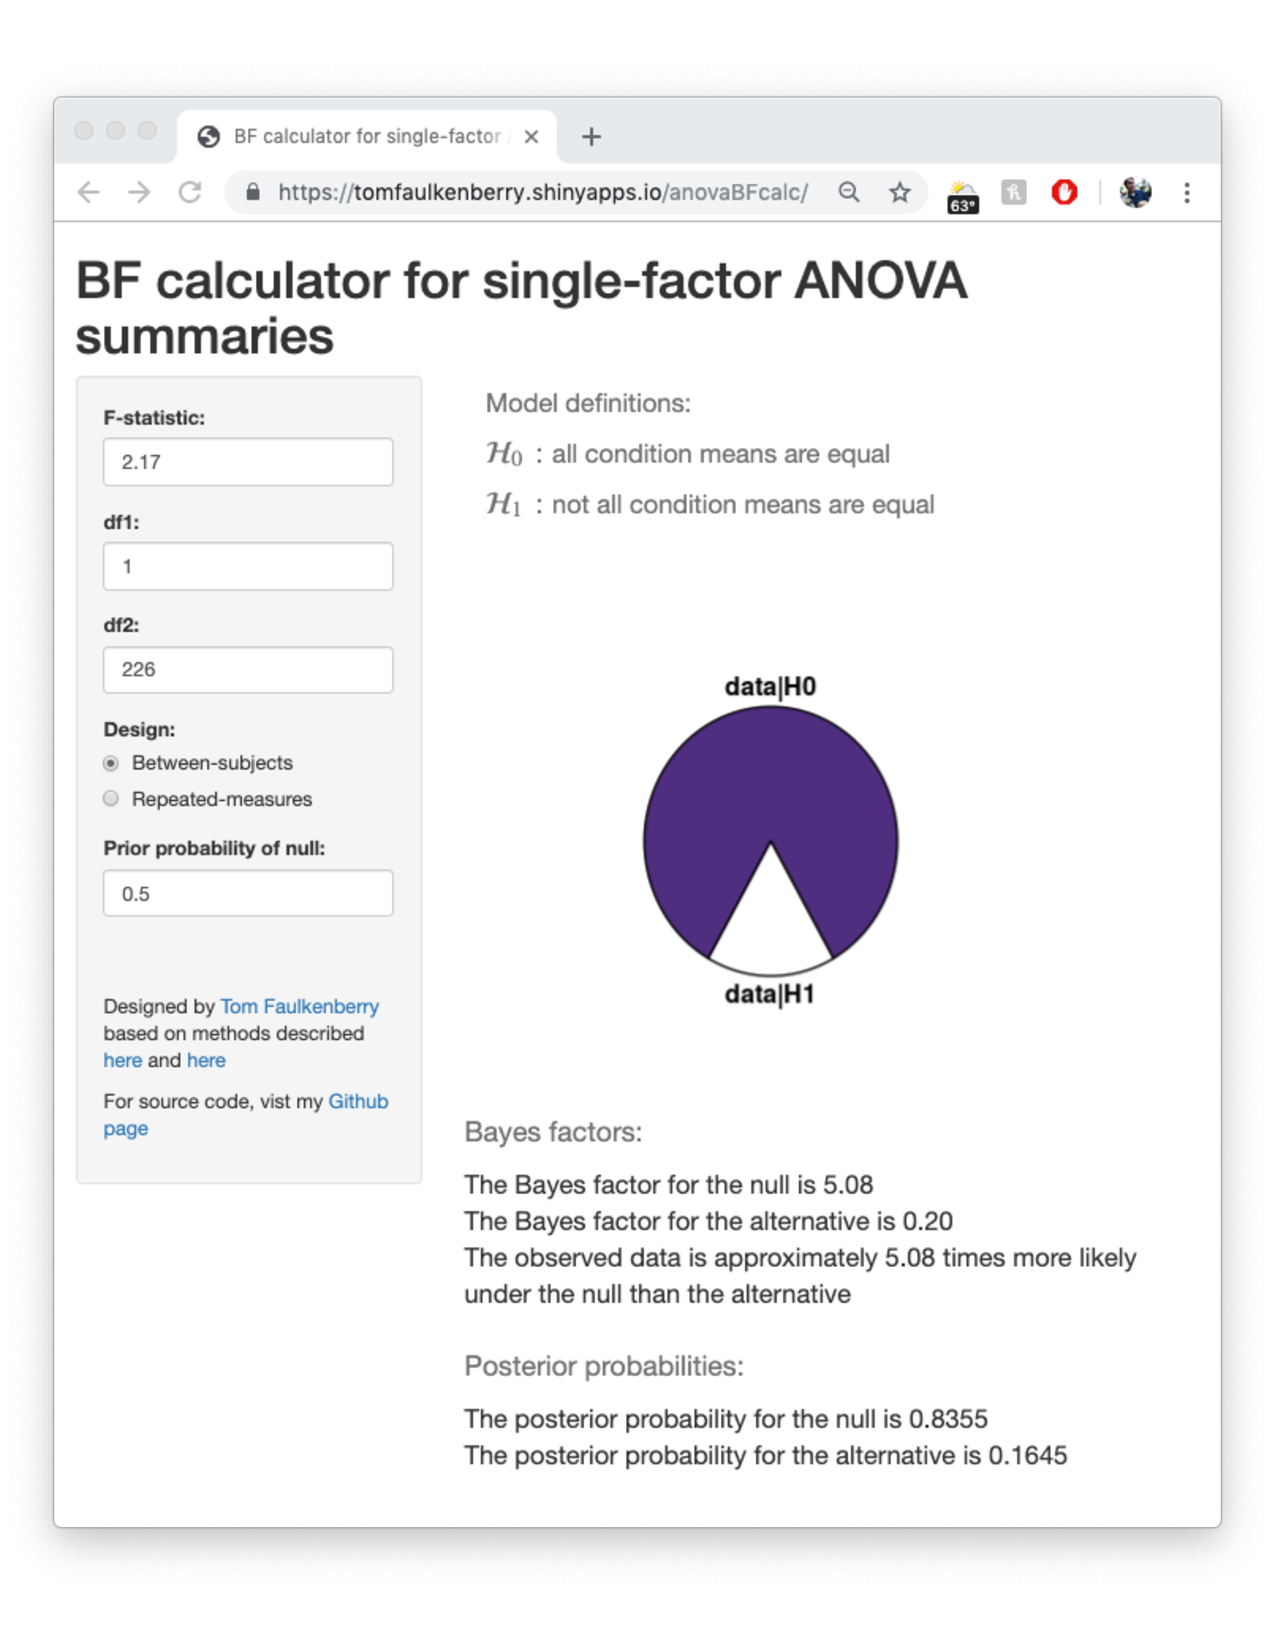
\includegraphics[width=0.75\textwidth]{fig1.pdf}
\caption{An interactive Bayes factor calculator, which can be accessed at \url{http://tomfaulkenberry.shinyapps.io/anovaBFcalc}. When provided minimal summary statistics from an ANOVA (e.g., the \(F\) statistic and the degrees of freedom), the calculator displays Bayes factors and posterior probabilities for \(\mathcal{H}_0\) and \(\mathcal{H}_1\), as well as a pizza plot showing the relative extent to which \(\mathcal{H}_0\) and \(\mathcal{H}_1\) predict the observed data. Note that the pizza plot reflects the Bayes factor, not the posterior probabilities of \(\mathcal{H}_0\) and \(\mathcal{H}_1\).}
\end{figure}

To illustrate the use of the online calculator, let us consider the following results from Rovenpor et al. (2019). In several experiments, Rovenpor et al. (2019) investigated whether violent conflict provides people with an enduring sense of meaning, thus perpetuating further intergroup conflict. In one study (Study 4), they measured perceptions of the scope of conflict as a function of whether participants first wrote about the conflict. Rovenpor et al. (2019) reported no significant difference between groups, \(F(1,226)=2.17\), \(p=0.143\). Though Rovenpor et al. (2019) interpreted this as a null effect, a strictly frequentist framework gives no indication of the degree of support for \(\mathcal{H}_0\). As Figure 1 displays, the Bayes factor calculator gives additional information that may help to assess the evidential value of this result. First, we see that \(B_{01}=5.08\), indicating that the observed data are approximately 5.08 times more likely under \(\mathcal{H}_0\) than \(\mathcal{H}_1\). Further, we see that the posterior probability for \(\mathcal{H}_0\) is 0.8355. That is, observing these data increases the plausibility of \(\mathcal{H}_0\) from 50\% (prior) to 83.55\% (posterior). The user can specify other values for the prior probability of \(\mathcal{H}_0\). For example, someone skeptical of the manipulation's effect might assign a high prior probability, say \(p(\mathcal{H}_0)=0.80\). The resulting posterior probability for \(\mathcal{H}_0\) is 0.9531; observing these data have \emph{increased} this user's belief in \(\mathcal{H}_0\). Alternatively, someone who believes the manipulation is effective might assign \(p(\mathcal{H}_0)=0.20\). In this case, the posterior probability for \(\mathcal{H}_0\) is 0.5595; this user's belief has also been shifted toward belief in \(\mathcal{H}_0\). Of course, this is a natural consequence of the Bayes factor, which by definition is the factor by which prior odds are multiplied after observing data. 

Sometimes, Bayesian reanalyses can reveal less evidence than might be originally thought. In Study 5 of Rovenpor et al. (2019), a large sample of participants (\(N=352\)) were randomly assigned to one of three conditions; in two of the non-control conditions, participants watched a video about a terrorist attack, one of which framed the attack as \enquote{meaningful}. Each participant was then given a series of questionnaire assessing perceptions of meaning in conflict. The authors reported a significant difference in perceived meaning of conflict, \(F(2,349)= 6.21\), \(p=0.002\). Traditionally, this would be viewed as support for \(\mathcal{H}_1\). However, the interactive Bayes factor calculator gives \(B_{10}=1.34\), indicating that the observed data is only 1.34 times more likely under \(\mathcal{H}_1\) than \(\mathcal{H}_0\). Equivalently, the plausibility of \(\mathcal{H}_1\) is only increased from 50\% (prior) to 57.22\% (posterior). The Bayesian reanalysis indicates that the observed data are not very evidential; that is, they do not sway belief toward either model very strongly.

In summary, the interactive Bayes factor calculator provides a useful supplement to the tools described by Ly et al. (2018) for assessing evidential value from studies. Like the JASP Summary Stats module, the calculator requires only minimal input, so it is easy for the user to obtain a measure of evidential value from minimal ANOVA summaries. In addition, the calculator provides interpretation of the Bayes factor, which may be useful to users who are new to using Bayesian inference (see also van Doorn et al., 2019).

One potential downside to the calculator is that the computations are based on a very specific choice of prior (the unit information prior). This prior is distributed over a large range of possible effects; on one hand, such a prior lets \enquote{the data speak for itself} (Gelman et al., 2013, p. 51), but on the other hand, the resulting Bayes factors are often inflated for \(\mathcal{H}_0\) and undersized for \(\mathcal{H}_1\). Because of this, one may wonder how the BIC prior performs compared to other default priors such as the JZS prior (Rouder, Morey, Speckman, \& Province, 2012). It turns out that the two approaches are quite comparable, as Faulkenberry (2018) demonstrated with a wide range of simulated datasets.

There are a few advantages that the calculator (and the BIC method more generally) provide over some existing options. One is that the calculator works for repeated measures designs. Though R users can use the \texttt{oneWayAOV.Fstat} function from the BayesFactor package (Morey \& Rouder, 2018) to calculate Bayes factors from summary statistics, this function only works for balanced, between-subjects designs. I will note that while the calculator works with unbalanced single-factor designs (in single factor designs, the \(SS\) calculations work out the same whether the design is balanced or unbalanced), it is currently an active area of investigation to see how these techniques extend to more general designs (unbalanced designs with multiple factors, etc.). In light of these comments, I think that the calculator will be useful to many people, especially as a supplement to the existing tools and emerging recommendations on conducting and reporting Bayesian analyses.

\subsection{Author Contributions}\label{author-contributions}

T. Faulkenberry is the sole author of this article and is responsible for its content.

\subsection{Declaration of Conflicting Interests}\label{declaration-of-conflicting-interests}

The author declared that there were no conflicts of interest with respect to the authorship or the publication of this article.

\subsection{Data, Materials, and Online Resources}\label{data-materials-and-online-resources}

The source code for the interactive Bayes factor calculator described in this paper can be accessed at \url{http://github.com/tomfaulkenberry/anovaBFcalc}.

\newpage

\section{References}\label{references}

\setlength{\parindent}{-0.5in}
\setlength{\leftskip}{0.5in}

\hypertarget{refs}{}
\leavevmode\hypertarget{ref-etz2017}{}%
Etz, A., \& Vandekerckhove, J. (2017). Introduction to Bayesian inference for psychology. \emph{Psychonomic Bulletin \& Review}, \emph{25}(1), 5--34. \url{https://doi.org/10.3758/s13423-017-1262-3}

\leavevmode\hypertarget{ref-faulkenberry2018}{}%
Faulkenberry, T. J. (2018). Computing Bayes factors to measure evidence from experiments: An extension of the BIC approximation. \emph{Biometrical Letters}, \emph{55}(1), 31--43. \url{https://doi.org/10.2478/bile-2018-0003}

\leavevmode\hypertarget{ref-faulkenberry2019}{}%
Faulkenberry, T. J. (2019). Estimating Bayes factors from minimal ANOVA summaries for repeated-measures designs. Retrieved from \url{https://arxiv.org/abs/1905.05569}

\leavevmode\hypertarget{ref-gelman}{}%
Gelman, A., Stern, H. S., Carlin, J. B., Dunson, D. B., Vehtari, A., \& Rubin, D. B. (2013). \emph{Bayesian Data Analysis} (3rd. ed.). Boca Raton, FL: Chapman; Hall/CRC.

\leavevmode\hypertarget{ref-jasp}{}%
JASP Team. (2018). JASP (Version 0.9){[}Computer software{]}. Retrieved from \url{https://jasp-stats.org/}

\leavevmode\hypertarget{ref-kass1995}{}%
Kass, R. E., \& Raftery, A. E. (1995). Bayes factors. \emph{Journal of the American Statistical Association}, \emph{90}(430), 773--795. \url{https://doi.org/10.1080/01621459.1995.10476572}

\leavevmode\hypertarget{ref-ly2018}{}%
Ly, A., Raj, A., Etz, A., Marsman, M., Gronau, Q. F., \& Wagenmakers, E.-J. (2018). Bayesian reanalyses from summary statistics: A guide for academic consumers. \emph{Advances in Methods and Practices in Psychological Science}, \emph{1}(3), 367--374. \url{https://doi.org/10.1177/2515245918779348}

\leavevmode\hypertarget{ref-masson2011}{}%
Masson, M. E. J. (2011). A tutorial on a practical Bayesian alternative to null-hypothesis significance testing. \emph{Behavior Research Methods}, \emph{43}(3), 679--690. \url{https://doi.org/10.3758/s13428-010-0049-5}

\leavevmode\hypertarget{ref-BF}{}%
Morey, R. D., \& Rouder, J. N. (2018). \emph{BayesFactor: Computation of bayes factors for common designs}. Retrieved from \url{https://CRAN.R-project.org/package=BayesFactor}

\leavevmode\hypertarget{ref-nathoo2016}{}%
Nathoo, F. S., \& Masson, M. E. J. (2016). Bayesian alternatives to null-hypothesis significance testing for repeated-measures designs. \emph{Journal of Mathematical Psychology}, \emph{72}, 144--157. \url{https://doi.org/10.1016/j.jmp.2015.03.003}

\leavevmode\hypertarget{ref-rouder2016}{}%
Rouder, J. N., Engelhardt, C. R., McCabe, S., \& Morey, R. D. (2016). Model comparison in ANOVA. \emph{Psychonomic Bulletin \& Review}, \emph{23}(6), 1779--1786. \url{https://doi.org/10.3758/s13423-016-1026-5}

\leavevmode\hypertarget{ref-rouder2012}{}%
Rouder, J. N., Morey, R. D., Speckman, P. L., \& Province, J. M. (2012). Default bayes factors for ANOVA designs. \emph{Journal of Mathematical Psychology}, \emph{56}(5), 356--374. \url{https://doi.org/10.1016/j.jmp.2012.08.001}

\leavevmode\hypertarget{ref-rovenpor2019}{}%
Rovenpor, D. R., O'Brien, T. C., Roblain, A., De Guissmé, L., Chekroun, P., \& Leidner, B. (2019). Intergroup conflict self-perpetuates via meaning: Exposure to intergroup conflict increases meaning and fuels a desire for further conflict. \emph{Journal of Personality and Social Psychology}, \emph{116}(1), 119--140. \url{https://doi.org/10.1037/pspp0000169}

\leavevmode\hypertarget{ref-vanDoorn2019}{}%
van Doorn, J., Bergh, D. van den, Bohm, U., Dablander, F., Derks, K., Draws, T., \ldots{} Evans, N. J. (2019). The JASP guidelines for conducting and reporting a Bayesian analysis. \url{https://doi.org/10.31234/osf.io/yqxfr}

\leavevmode\hypertarget{ref-wagenmakers2007}{}%
Wagenmakers, E.-J. (2007). A practical solution to the pervasive problems of \(p\)- values. \emph{Psychonomic Bulletin \& Review}, \emph{14}(5), 779--804. \url{https://doi.org/10.3758/bf03194105}

\leavevmode\hypertarget{ref-wagenmakers2017}{}%
Wagenmakers, E.-J., Love, J., Marsman, M., Jamil, T., Ly, A., Verhagen, J., \ldots{} Morey, R. D. (2017). Bayesian inference for psychology. Part II: Example applications with JASP. \emph{Psychonomic Bulletin \& Review}, \emph{25}(1), 58--76. \url{https://doi.org/10.3758/s13423-017-1323-7}


\end{document}
